% Chapter 3
\chapter{Machine Learning} % Main chapter title

\label{Chapter3} % For referencing the chapter elsewhere, use \ref{Chapter1}

\lhead{Chapter 3. \emph{Random Forest Machine Learning}} % This is for the header on each page - perhaps a shortened title

%----------------------------------------------------------------------------------------
\section{Decision Tree}

\begin{compactitem}

\item {Introduction to Classification and Regression Trees (CART)}
Decision Trees are commonly used in data mining with the objective of creating a model that predicts the value of a target (or dependent variable) based on the values of several input (or independent variables).  In today's post, we discuss the CART decision tree methodology.  The CART or Classification and Regression Trees methodology was introduced in 1984 by Leo Breiman, Jerome Friedman, Richard Olshen and Charles Stone as an umbrella term to refer to the following types of decision trees:\cite{blog-CART-Intro}

\item {Classification Trees}: where the target variable is categorical and the tree is used to identify the "class" within which a target variable would likely fall into.

\begin{figure}[ht]
  \centering
	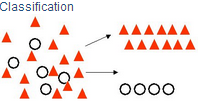
\includegraphics[width=0.7\textwidth, keepaspectratio=true]{chap3-Classification.png}
  \caption{classification tree.}
  \label{fig:chap3-Classification}
\end{figure}

\item {Regression Trees}: where the target variable is continuous and tree is used to predict it's value.
\begin{figure}[ht]
  \centering
    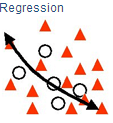
\includegraphics[width=0.7\textwidth, keepaspectratio=true]{chap3-Regression.png}
  \caption{Regression tree.}
  \label{fig:chap3-Regression}
\end{figure}

The CART algorithm is structured as a sequence of questions, the answers to which determine what the next question, if any should be.  The result of these questions is a tree like structure where the ends are terminal nodes at which point there are no more questions.  A simple example of a decision tree is as follows \autoref{fig:chap3-CART_tree_titanic_survivors}:
\begin{figure}[ht]
  \centering
    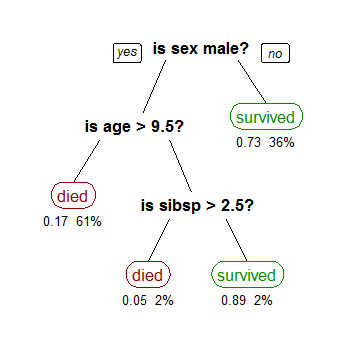
\includegraphics[width=0.7\textwidth, keepaspectratio=true]{chap3-CART_tree_titanic_survivors.png}
  \caption{A tree showing survival of passengers on the Titanic ("sibsp" is the number of spouses or siblings aboard). The figures under the leaves show the probability of survival and the percentage of observations in the leaf.}
  \label{fig:chap3-CART_tree_titanic_survivors}
\end{figure}

\end{compactitem}

\section{Ensemble Learning}
Ensemble methods are learning algorithms that construct a set of classifiers and then classify
new data points by taking a (weighted) vote of their predictions. The more recent algorithms include error-correcting output coding, Bagging and boosting.
\cite{Dietterich:2000:EMM:648054.743935}

\begin{compactitem}

\item {Introduction}
\autoref{fig:chap3-prob}

\begin{figure}[ht]
  \centering
	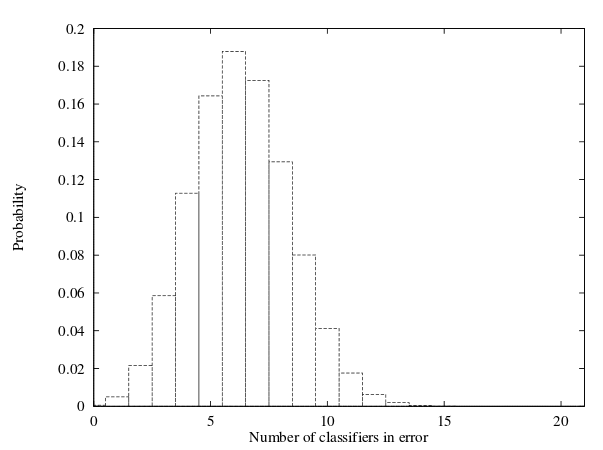
\includegraphics[width=0.7\textwidth, keepaspectratio=true]{chap3-prob.png}
  \caption{The probability that exactly l of 21 hypotheses will make an error, assuming each hypothesis has an
	error rate of 0.3 and makes its errors independently of the other hypotheses. }
  \label{fig:chap3-prob}
\end{figure}

\item {Three fundamental reasons}
\autoref{fig:chap3-ThreeReasons}

\begin{figure}[ht]
  \centering
    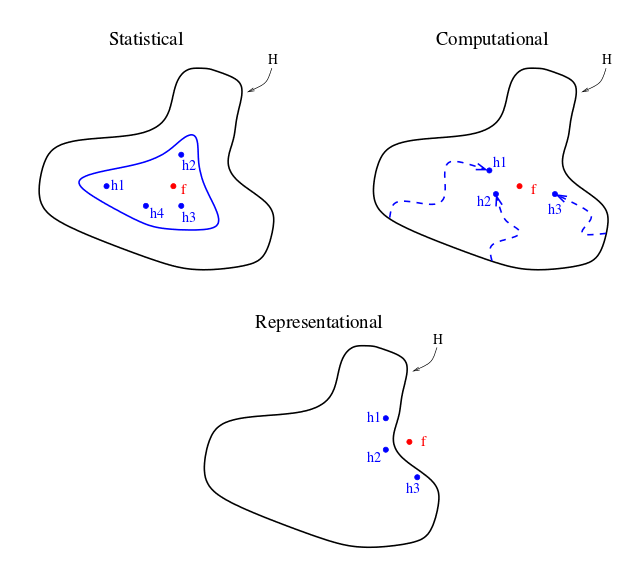
\includegraphics[width=0.7\textwidth, keepaspectratio=true]{chap3-ThreeReasons.png}
  \caption{The fundamental resons why an ensemble may work better than a single classifier. }
  \label{fig:chap3-ThreeReasons}
\end{figure}

\end{compactitem}

\section{Random Forest}

Random forests are examples of ensemble learning methods which combine predictions of weak classifiers.
We use Breiman’s Random Forest Machine Learning Algorithm \cite {Statistics01randomforests} \cite{Frederick-Livingston} to train the classifiers.
\begin{compactitem}
\item {Introduction}
A classical machine learner is developed by collecting samples of data to represent the entire population. 
This data set is usually subdivided into two or more dataset. One Part of the dataset set is commonly use for developing the machine learner(training data set), and the remaining data is use for evaluation( testing data set to verify the learned model). 
Often this data set is imbalanced; the data consists of only a very small minority of the data. Imbalanced machine learners tend to perform poorly with the classification. 
During the testing phase these rare cases are unseen during the training phase and are usually misclassified. 
Leo Breiman, a statistician from University of California at Berkeley, developed a machine learning algorithm to improve classification of diverse data using random sampling and random  attributes/features selection.

\item {Background}
The random forest machine learner, is a meta-learner; meaning consisting of many individual learners (trees). The random forest uses multiple random trees classifications to votes on an overall classification for the given set of inputs.
In Breiman’s later work, this algorithm was modified to perform both un-weighted and weighted voting. 
The forest chooses the classification that contains the most votes. \autoref{fig:chap3-meta-learners}. below is a visual representation of the un-weighted random forest algorithm.

\begin{figure}[ht]
  \centering
    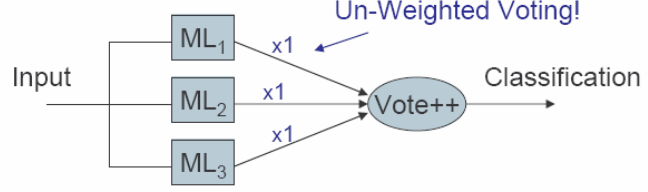
\includegraphics[width=0.7\textwidth, keepaspectratio=true]{chap3-meta-learners.png}
  \caption{Meta Learners}
  \label{fig:chap3-meta-learners}
\end{figure}

\item {Bootstrap}

\item {Bagging : sampling with replacement members}
\begin{figure}[ht]
  \centering
    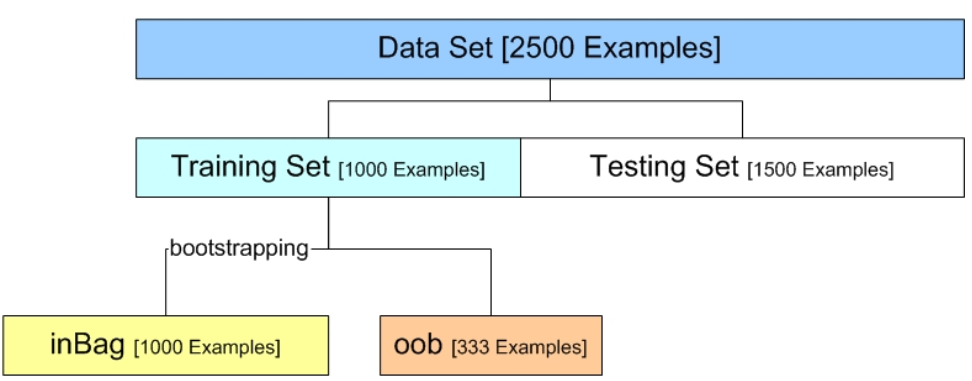
\includegraphics[width=0.7\textwidth, keepaspectratio=true]{chap3-SampleWithReplacing.png}
  \caption{Sample with Replacing}
  \label{fig:chap3-SampleWithReplacing}
\end{figure}

\item {Build Tree}
\item {Ensemble}
\item {Out Of Bag Error Estimate}

\end{compactitem}

\section{Adaboost}
\label{app:abr}
The pseudo-code of Adaboost. For details see \cite{Freund99ashort}.

\begin{figure}[bth]
  \begin{center}
    \begin{center}
      \fbox{\parbox{11.4cm}{\small\sffamily {\bf Algorithm AdaBoost}$({\bf Z}, T)$
          \begin{itemize}
          \item[] {\bf Input:} $l$ examples ${\bf Z}=\langle ({\bf x}_1,y_1), \ldots,
            ({\bf x}_l,y_l)\rangle$
          \item[] {\bf Initialize:} $w_{1}({\bf z}_i) = 1/l$ for all $i=1\ldots l$
          \item[] {\bf Do for} $t=1,\ldots,T$,
            \begin{enumerate}
            \item Train classifier with respect to the weighted sample set
              $\{{\bf Z},{\bf w}^t\}$ and \\ obtain hypothesis $h_t:{\bf x}\mapsto \{\pm 1\}$
            \item Calculate the training error $\epsilon_t$ of $h_{t}$:
              \begin{equation}
                \label{epsilon_t}
                \epsilon_{t}=\sum_{i=1}^{l} w^t({\bf z}_i)\Ind(h_t({\bf x}_i)\not=y_i)~,
              \end{equation}
              abort if $\epsilon_t=0$ or $\epsilon_t\geq \frac{1}{2}-\Delta$, where
              $\Delta$ is a small constant
            \item Set
              \begin{equation}
                \label{def_b_t}
                b_t = \log\frac{1-\epsilon_{t}}{\epsilon_{t}}.
              \end{equation}
            \item Update weights ${\bf w}^t$:
              \begin{equation}
                \label{update_w}
                w^{t+1}({\bf z}_i) = w^t({\bf z}_i)\exp\left\{-b_t
                \Ind(h_t({\bf x}_i)=y_i)\right\}/Z_t~,
              \end{equation}
              where $Z_t$ is a normalization constant, such that $\sum_{i=1}^l
              w_{t+1}({\bf z}_i)=1$.
            \end{enumerate}
          \item[]{\bf Output:} Final hypothesis
            \begin{equation}
              \label{fin_hyp}
              f({\bf x}) = \sum_{t=1}^{T} c_t h_{t}({\bf x}), \quad \mbox{where} \quad c_t:=\frac{b_t}{\sum_{t=1}^T |b_t|}
            \end{equation}
          \end{itemize}
          } 
          }
    \end{center}
  \end{center}
  \caption[]{The AdaBoost algorithm \cite{Freund99ashort}.\label{fig:ABALG}}
\end{figure}

%----------------------------------------------------------------------------------------

